\documentclass[a4paper,11pt,dvipdfmx]{jsarticle}


% 数式
\usepackage{amsmath,amsfonts}
\usepackage{bm}

% 画像
\usepackage[dvipdfmx]{graphicx}
\usepackage{framed}

% 図形
\usepackage{tikz}
\usetikzlibrary{shapes.geometric}
\usetikzlibrary {shapes.misc}

% ソースコード
\usepackage{listings,jlisting,color}
\lstset{
basicstyle={\ttfamily},
identifierstyle={\small},
commentstyle={\smallitshape},
keywordstyle={\small\bfseries},
ndkeywordstyle={\small},
stringstyle={\small\ttfamily},
frame={tb},
breaklines=true,
columns=[l]{fullflexible},
numbers=left,
xrightmargin=0zw,
xleftmargin=3zw,
numberstyle={\scriptsize},
stepnumber=1,
numbersep=1zw,
lineskip=-0.5ex
}
\renewcommand{\lstlistingname}{ソースコード}


\begin{document}
\definecolor{shadecolor}{gray}{0.70}

\title{数値計算 Class-11 演習}
\author{21T2166D 渡辺大樹}
\date{\today}
\maketitle

\section{演習内容}
Class-11では前回行った基本関数の複数の組み合わせモデルによる補間関数の作成を、誤差の小さいものを自動的に選択して作成する、前方選択について演習していく。

今回新規に用いたコードをソースコード\ref{main},\ref{for.h},\ref{py}に示す。長くなるためpdf末尾に記載している。

以下ではどういった方法で誤差の小さい補間関数を自動で作成していくかを解説していく。

切り口としては誤差の小さい補間関数をどのように取得すべきか、というところにある。基本関数の組み合わせ総数が少ない
場合、全探索(すべてのパターンで試す)すればよいが、基本関数の組み合わせが多くなってしまうと計算量は階乗のオーダーになり
爆発的に大きくなってしまう。これを解決し、かつ最適な補間関数を作成するための手法が前方選択になる。
この手法は機械学習などにも使われるものである。

この手法はシンプルで、n個の基本関数をそれぞれ1つずつ選び、最小二乗法でデータの補間関数を作る。(図\ref{f1})

\begin{figure}[htbp]
    \centering
    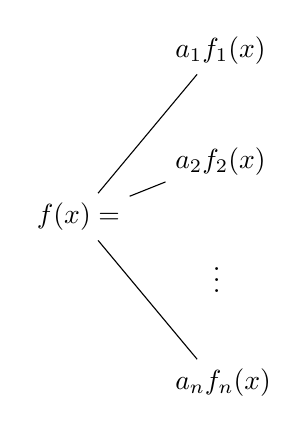
\begin{tikzpicture}[
        level 1/.style={sibling distance=40pt, level distance=50pt},
        every node/.style={text centered},
        TreeNode/.style={text width=30pt},
        func/.style={text width=30pt},
    ]
    \node[TreeNode](a) {$f(x)=$}[grow=right]
        child {
            node[func](b) {$a_nf_n(x)$}
            edge from parent
                node[right] {}
        }
        child {
            node{$\vdots$}
            edge from parent[draw=none]
        }
        child {
            node[func](c) {$a_2f_2(x)$}
        }
        child {
            node[func](d) {$a_1f_1(x)$}
        };
    \end{tikzpicture}
    \caption{n個の基本関数からそれぞれ補間関数を作成}
    \label{f1}
\end{figure}

出来た補間関数の誤差をそれぞれ計算し、一番小さくなった基本関数を選択する。(図\ref{f2})

\begin{figure}[htbp]
    \centering
    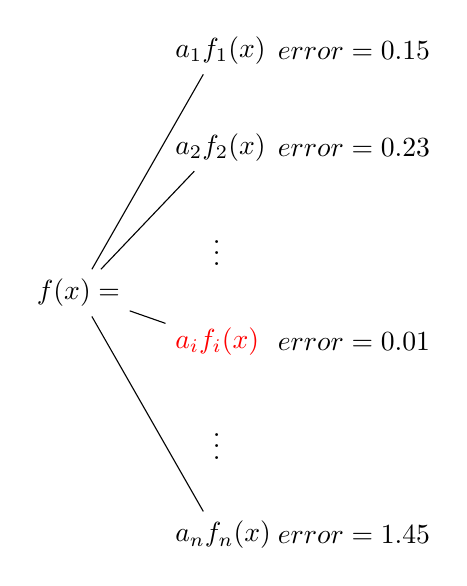
\begin{tikzpicture}[
        level 1/.style={sibling distance=35pt, level distance=50pt},
        every node/.style={text centered},
        TreeNode/.style={text width=30pt},
        func/.style={text width=30pt},
    ]
    \node[TreeNode](root) {$f(x)=$}[grow=right]
        child {
            node[func](n) {$a_nf_n(x)$}
            edge from parent
                node[right] {}
        }
        child {
            node{$\vdots$}
            edge from parent[draw=none]
        }
        child {
            node[func][red](i) {$a_if_i(x)$}
        }
        child {
            node {$\vdots$}
            edge from parent[draw=none]
        }
        child {
            node[func](2) {$a_2f_2(x)$}
        }
        child {
            node[func](1) {$a_1f_1(x)$}
        };

        \node also [label=right:{$error = 0.15$}] (1);
        \node also [label=right:{$error = 0.23$}] (2);
        \node also [label=right:{$error = 0.01$}] (i);
        \node also [label=right:{$error = 1.45$}] (n);
    \end{tikzpicture}
    \caption{n個の補間関数の誤差から一番小さいものを選択}
    \label{f2}
\end{figure}

ここからこの関数の続きを今と同じように生成していく。$f_i$以外の基本関数で前回生成した関数の続きを最小二乗法で補間し
誤差の小さい補間関数を選択する(図\ref{f3})。

\begin{figure}[htbp]
    \centering
    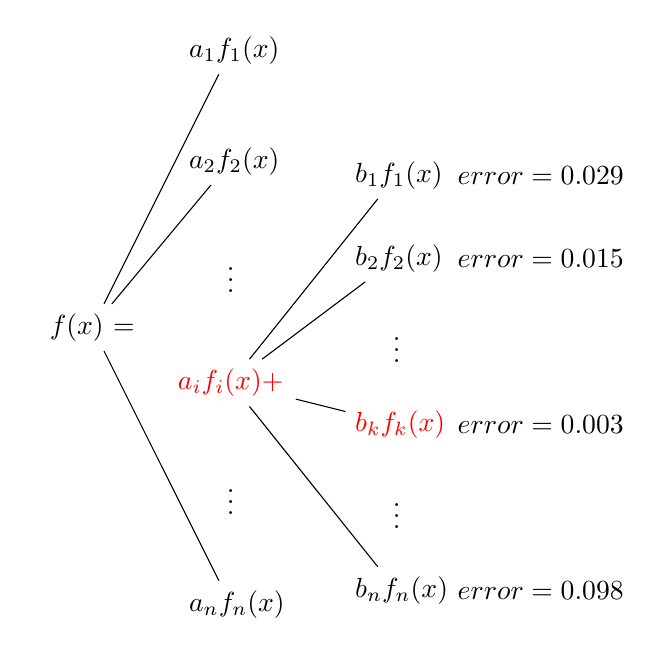
\begin{tikzpicture}[
        level 1/.style={sibling distance=40pt, level distance=50pt},
        level 2/.style={sibling distance=30pt, level distance=60pt},
        every node/.style={text centered},
        TreeNode/.style={text width=40pt},
        func/.style={text width=30pt},
    ]
    \node[TreeNode](a) {$f(x)=$}[grow=right]
        child {
            node[func](n) {$a_nf_n(x)$}
        }
        child {
            node{$\vdots$}
            edge from parent[draw=none]
        }
        child {
            node[TreeNode][red](i) {$a_if_i(x)+$}
            child{node[func](2_n) {$b_nf_n(x)$}}
            child{
                node {$\vdots$}
                    edge from parent[draw=none]
            }
            child{node[func][red](2_k) {$b_kf_k(x)$}}
            child{
                node {$\vdots$}
                    edge from parent[draw=none]
            }
            child{node[func](2_2) {$b_2f_2(x)$}}
            child{node[func](2_1) {$b_1f_1(x)$}};
        }
        child {
            node {$\vdots$}
            edge from parent[draw=none]
        }
        child {
            node[func](2) {$a_2f_2(x)$}
        }
        child {
            node[func](1) {$a_1f_1(x)$}
        };
        \node also [label=right:{$error = 0.029$}] (2_1);
        \node also [label=right:{$error = 0.015$}] (2_2);
        \node also [label=right:{$error = 0.003$}] (2_k);
        \node also [label=right:{$error = 0.098$}] (2_n);
    \end{tikzpicture}
    \caption{n-1個($f_i$以外)の基本関数でそれぞれ補間し誤差の小さいものを選択}
    \label{f3}
\end{figure}

これを繰り返していくことで、計算量は抑えられつつも最適な補間関数を得ることができる。

実際に\ref{for.h}にはこのアルゴリズムが実装されている。

\section{演習結果-考察}
以下では前回も用いた6つのデータセットでこの前方選択と補間を行った結果を示す。

\subsection{example2.txt}
初めにデータセットexample2.txtで行った結果を図\ref{ex2}に示す。
\begin{figure}[h]
\centering
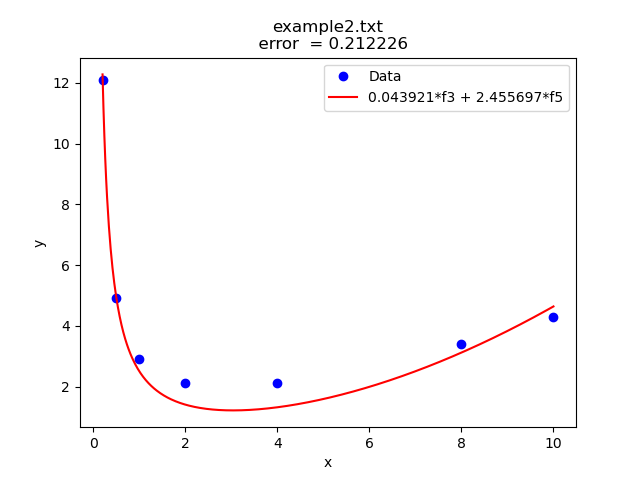
\includegraphics[width=80mm]{c:/program_code/NumMeth/Class11STU/code/plot_example2.txt.png}
\caption{example2.txtでのデータ点と補間関数}
\label{ex2}
\end{figure}

見切れてしまっているが図\ref{ex2}での補間モデルは\[f(x)=0.016x^3 -0.189x^2 + 0.984x + \frac{2.469}{x} -0.000e^x -0.441\]
となった。$e^x$の係数は表記上0であるが$10^{-5}$程の係数である。誤差は0.00097となった。

前回行ったモデルセットによる選択的な補間では、一番誤差の小さい場合でも補間モデルが$f(x)=0.001x^2+0.381x+\frac{2.403}{x}$
であり誤差は0.0072と今回の補間モデルではその関数が複雑になったことで誤差も縮まっていることが分かる。

\subsection{nh\_bb\_age\_length.txt}
続いてデータセットnh\_bb\_age\_length.txtで行った結果を図\ref{len}に示す。
\begin{figure}[h]
\centering
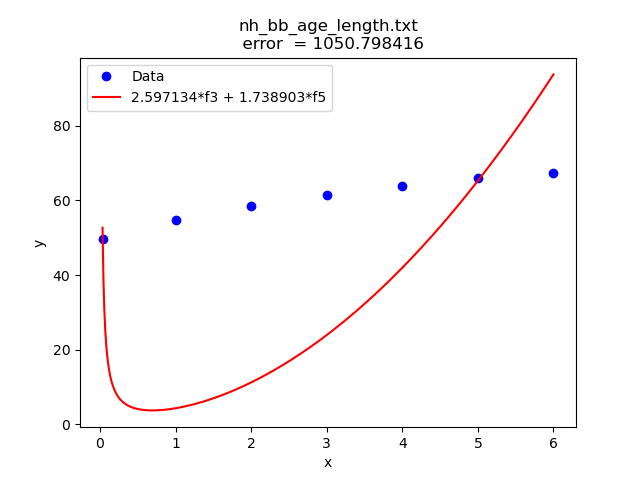
\includegraphics[width=80mm]{c:/program_code/NumMeth/Class11STU/code/plot_nh_bb_age_length.txt.png}
\caption{nh\_bb\_age\_length.txtでのデータ点と補間関数}
\label{len}
\end{figure}

これも図では見切れているが補間モデルは
\[f(x)=0.003x^3 -0.276x^2 + 4.367x - \frac{0.036}{x} -0.001e^x + 50.748\]
となった。誤差は0.0003となった。

これも前回行った補間では誤差が0.039ほどだったためおよそ$\frac{1}{100}$も誤差が小さくなったことが分かる。

\subsection{nh\_bb\_age\_weigth.txt}
続いてデータセットnh\_bb\_age\_weigth.txtで行った結果を図\ref{wgh}に示す。
\begin{figure}[h]
\centering
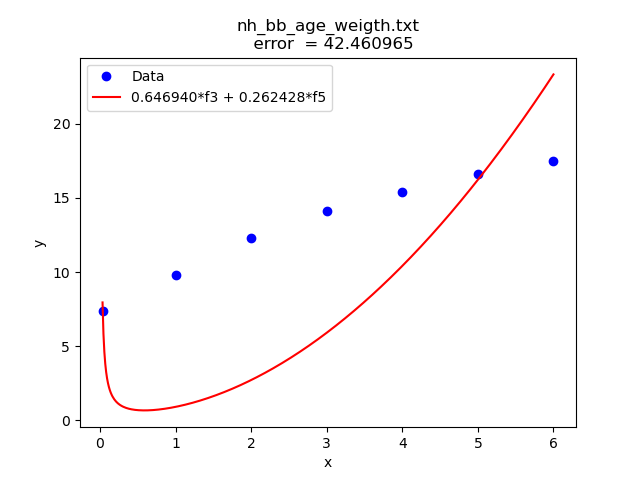
\includegraphics[width=80mm]{c:/program_code/NumMeth/Class11STU/code/plot_nh_bb_age_weigth.txt.png}
\caption{nh\_bb\_age\_weigth.txtでのデータ点と補間関数}
\label{wgh}
\end{figure}

補間モデルは
\[f(x)= 0.071x^3 - 0.792x^2 + 4.440x + \frac{0.040}{x} - 0.005e^x+ 6.051\]
となり、誤差は0.0002となった。

これも前回行った補間では誤差が0.009だったため前回の補間よりもより精度のよい補間ができていることが分かる。

\subsection{nh\_covid-italy.txt}
続いてデータセットnh\_covid-italy.txtで補間を行った結果を図\ref{cov}に示す。
\begin{figure}[h]
\centering
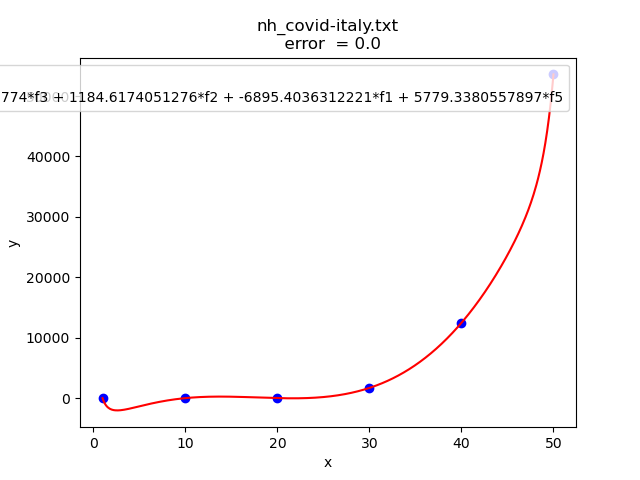
\includegraphics[width=80mm]{c:/program_code/NumMeth/Class11STU/code/plot_nh_covid-italy.txt.png}
\caption{nh\_covid-italy.txtでのデータ点と補間関数}
\label{cov}
\end{figure}

図\ref{cov}の補間モデルは
\[f(x) = 1.255x^3 + -67.807x^2 + 1184.617x + \frac{5779.338}{x} + 0.000e^x - 6895.404\]
となった。誤差は0.0と非常に小さく、\ref{main}を実行したときに出力されたデータファイルを見てもほとんど0に近い値になっている。

これも前回行った補間では誤差は$3.1\cdot 10^6$ほどだったため一気に精度が上がったことが分かる。

ただこの図\ref{cov}を見ると一つ目のデータ点のすぐ後の補間関数が少し下に下がっている。
このデータはおそらくイタリアのコロナ感染者についてのデータであると思うが実際に感染者の増加がこの通りであるわけではない可能性が高い。

補間モデルの精度を上げることはもちろんメリットもあるが、この例のように必ずしも誤差の小さな補間モデルが優れているわけではないと考えられる。

\subsection{nh\_fish.txt}
続いてデータセットnh\_fish.txtで補間を行った結果を図\ref{fish}に示す。
\begin{figure}[h]
\centering
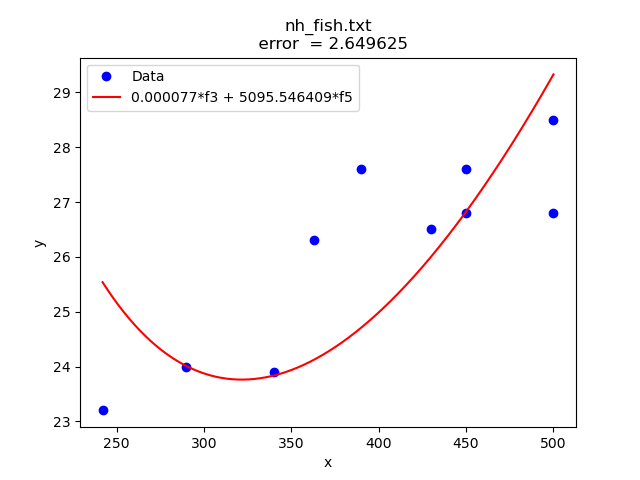
\includegraphics[width=80mm]{c:/program_code/NumMeth/Class11STU/code/plot_nh_fish.txt.png}
\caption{nh\_fish.txtでのデータ点と補間関数}
\label{fish}
\end{figure}

図\ref{fish}の補間モデルは
\[f(x) = 0.000x^3 - 0.003x^2 + 1.902x + \frac{42273.604}{x} -450.301\]
となった。データ点のばらつきのせいか$e^x$の項は最小二乗法の結果がうまく出なかったため項が入っていない。
誤差は0.534となった。

前回行った補間での誤差は0.564で、確かに今回は小さくなっているがこれまでの演習結果と比較するとあまり変わらないように見える。
これはおそらくデータのばらつきが大きいため正確な関数の近似が難しいことが要因に挙げられる。
こういったばらつきのあるデータは、その関係を示したいのなら正確で誤差のない複雑なモデルの補間よりも、
シンプルな一次関数や対数関数での最小二乗法などでの補間が適していると考えられる。

\subsection{nh\_wine.txt}
最後にデータセットnh\_wine.txtで補間を行った結果を図\ref{wine}に示す。
\begin{figure}[h]
\centering
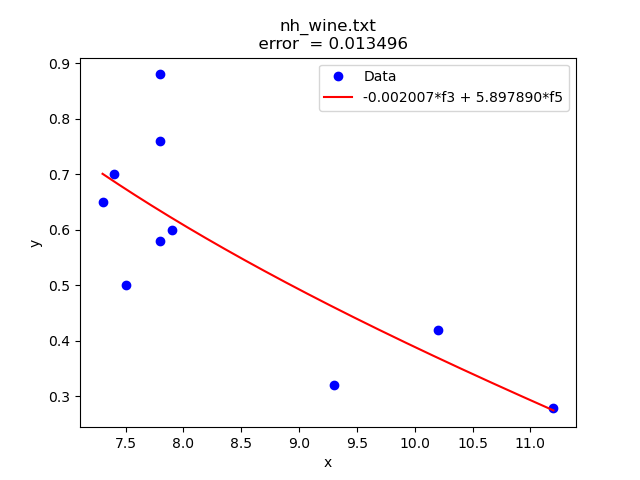
\includegraphics[width=80mm]{c:/program_code/NumMeth/Class11STU/code/plot_nh_wine.txt.png}
\caption{nh\_wine.txtでのデータ点と補間関数}
\label{wine}
\end{figure}

図\ref{wine}の補間モデルは
\[f(x) = -1.891x^3 - 0.000x^2  - \frac{514.318}{x} - 0.000e^x -126.840\]
となった。こちらも6回目の選択でLU分解出来ない係数行列が出来てしまったようで$x$の項がなくなっている。
誤差は0.0094となった。

前回の補間での誤差は0.0131であり2.5でのデータセット同様あまり変化の少ない結果となった。理由も2.5と同じく、
データのばらつきが起因しているものと考えられる。

\lstinputlisting[caption=main\_forward\_selection.c, label=main]{C:/Program_Code/NumMeth/Class11STU/code/main_forward_selection.c}
\lstinputlisting[caption=forward\_selection.h, label=for.h]{C:/Program_Code/NumMeth/Class11STU/code/forward_selection.h}
\lstinputlisting[caption=fig.py, label=py]{C:/Program_Code/NumMeth/Class11STU/code/fig.py}


\end{document}